\documentclass[tikz,border=10pt]{standalone}
\usepackage{tikz}
\usetikzlibrary{calc,patterns,decorations,decorations.pathreplacing,shapes.arrows}

\begin{document}

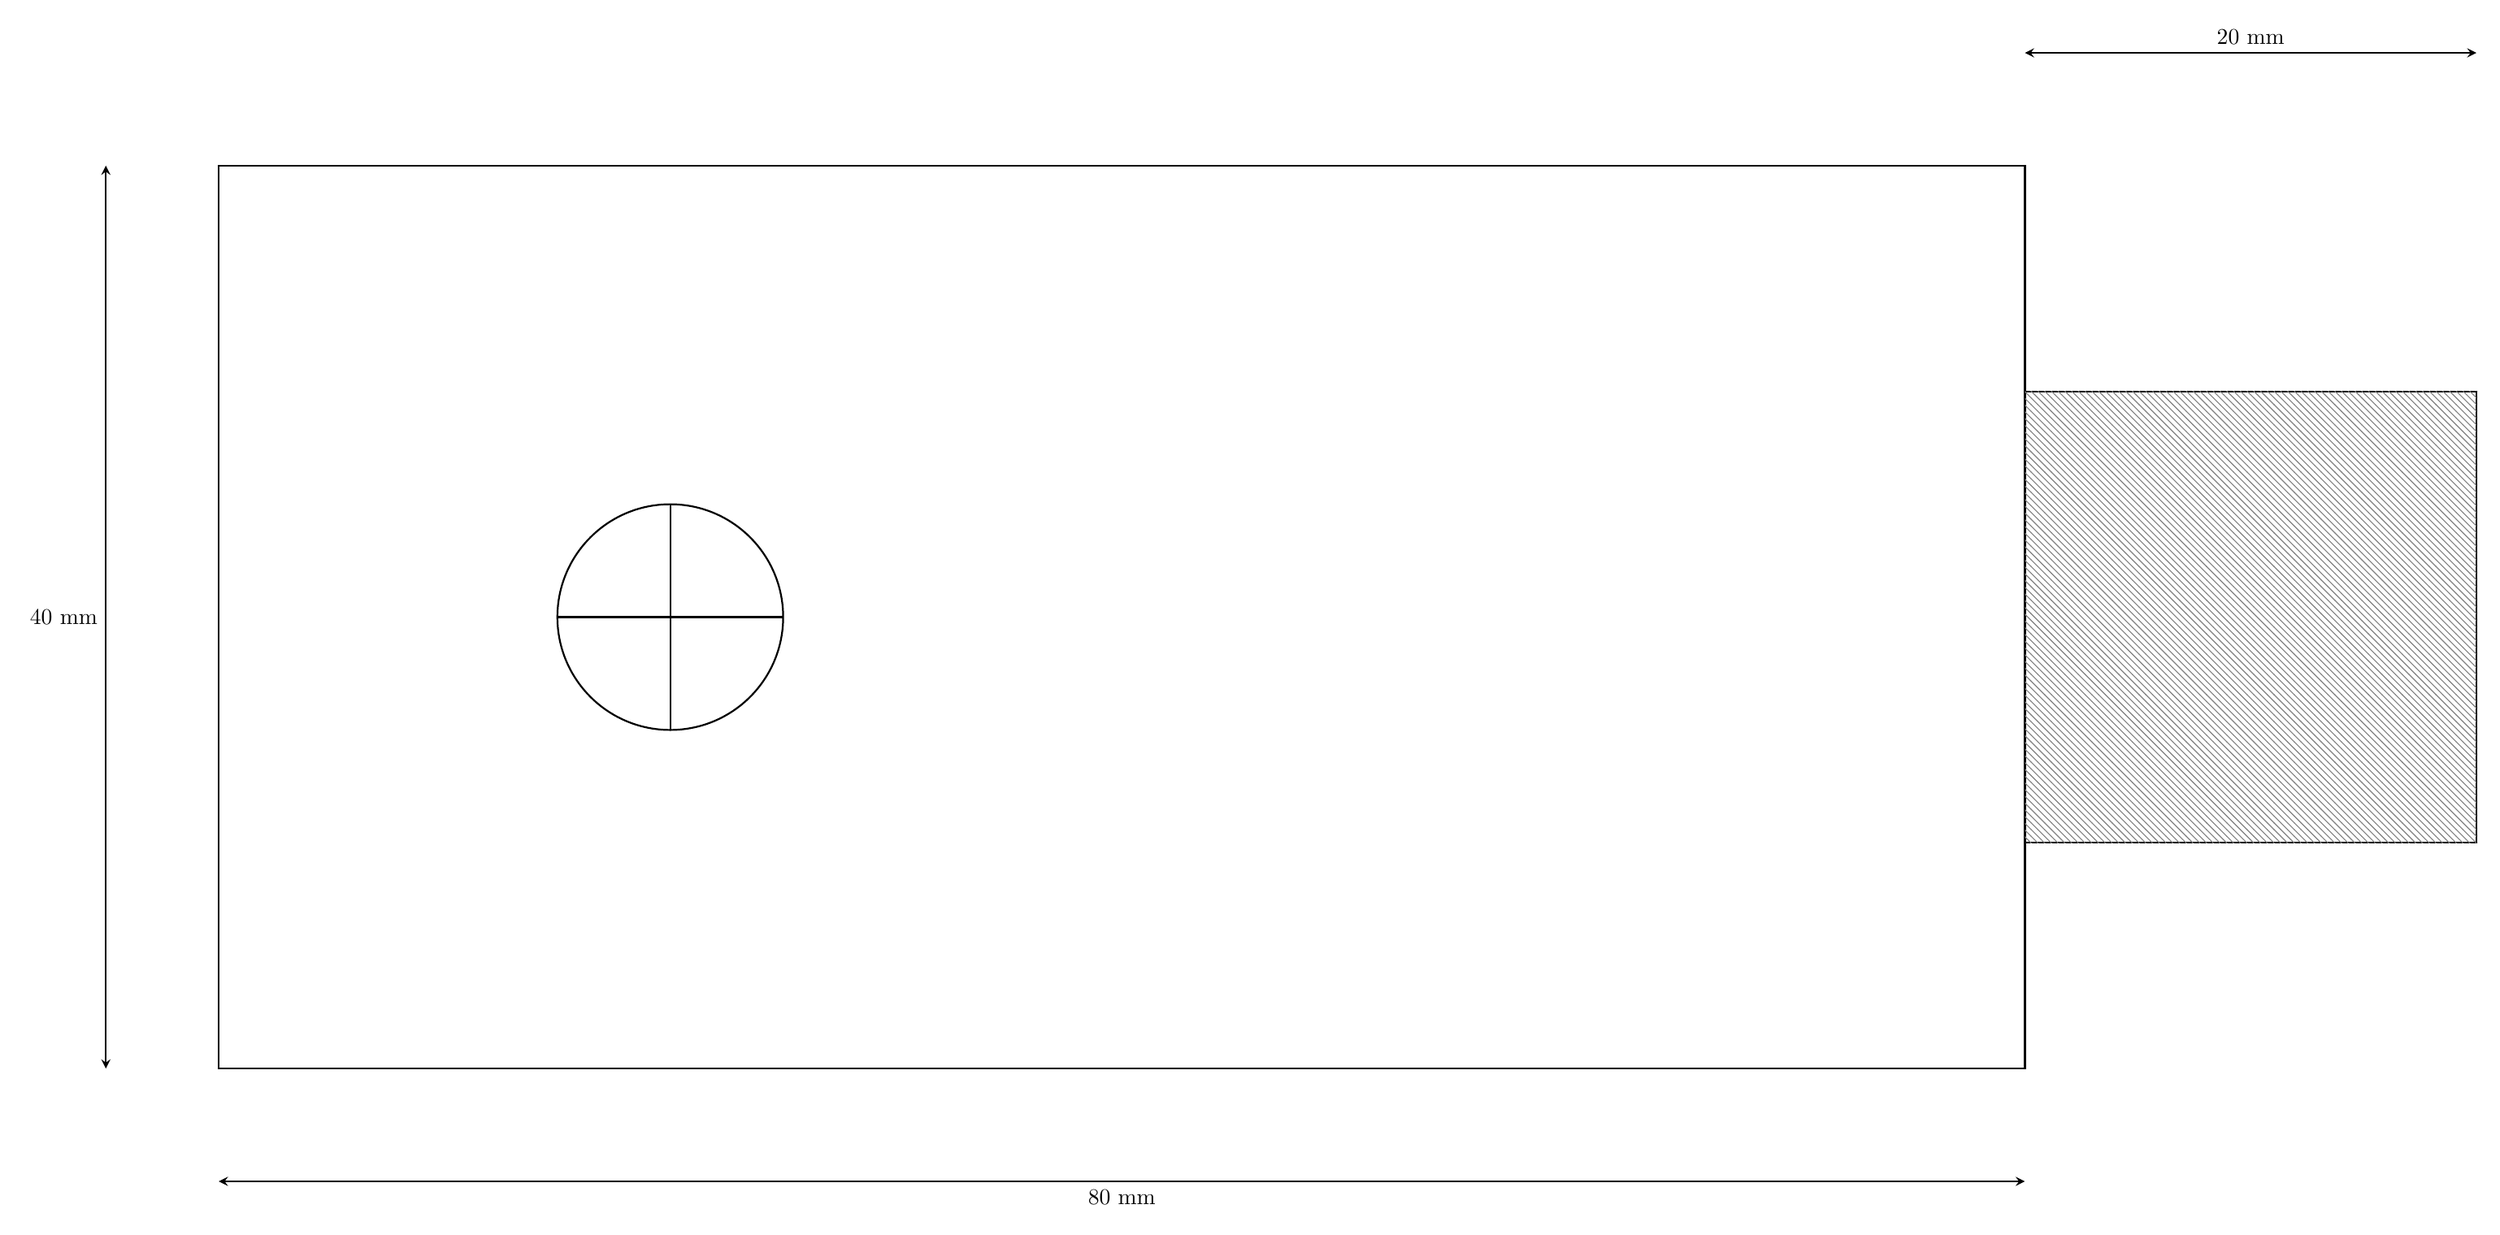
\begin{tikzpicture}[scale=0.35278]  % Scale factor to convert mm to TikZ units (1 pt = 0.35278 mm)

    % Define some common styles
    \tikzset{
        dimline/.style={thick, >=stealth},
        hidden/.style={dashed},
        section/.style={pattern=north west lines, pattern color=black!50}
    }
    
    % Draw the base rectangle (main body) - 80 mm × 40 mm
    \draw[thick] (0,0) rectangle (80,40);
    
    % Draw a circular hole (Diameter: 10 mm)
    \draw[thick] (20,20) circle (5);
    
    % Draw a side extension (20 mm × 20 mm)
    \draw[thick] (80,10) -- (100,10) -- (100,30) -- (80,30);
    
    % Add hidden lines (dashed) - Center of the hole
    \draw[hidden] (20,15) -- (20,25);
    
    % Dimension lines
    \draw[dimline,<->] (0,-5) -- (80,-5) node[midway, below] {80 mm};
    \draw[dimline,<->] (-5,0) -- (-5,40) node[midway, left] {40 mm};
    \draw[dimline,<->] (80,45) -- (100,45) node[midway, above] {20 mm};
    
    % Center mark for the hole
    \draw[dimline] (20,15) -- (20,25);
    \draw[dimline] (15,20) -- (25,20);
    
    % Section pattern (Hatching)
    \fill[section] (80,10) rectangle (100,30);

\end{tikzpicture}

\end{document}
